\chapter{Maximum Acceleration Limited Path Following Method}
\label{ch:appendix_max_accel}

This is a relaxed maximum acceleration (in path parallel, and orthogonal directions) calculation-based vector field, where we assume that a vehicle approaching at $V_{approach}$ accelerates at the highest possible acceleration to achieve $V_{path}$ while converging to the path.

%%%%%%%%%%%%%%%%%%%%%%%%%%%%%%%%%%%%%%%%%%%5
% ORTHOGONAL VELOCITY
\section{Defining orthogonal velocity curve}

The 'orthogonal' velocity is what actually ties the 'time' - 'track error' relationship ($e(t)$) since the cross track error is only affected by the orthogonal velocity. Theoretically, 'parallel' velocity can have an infinite number of plausible $e(t)$ curves.\newline

Let's take a close look at a typical orthogonal velocity curve in \autoref{fig:v_orth_curve}.

\begin{figure}[h]
\centering
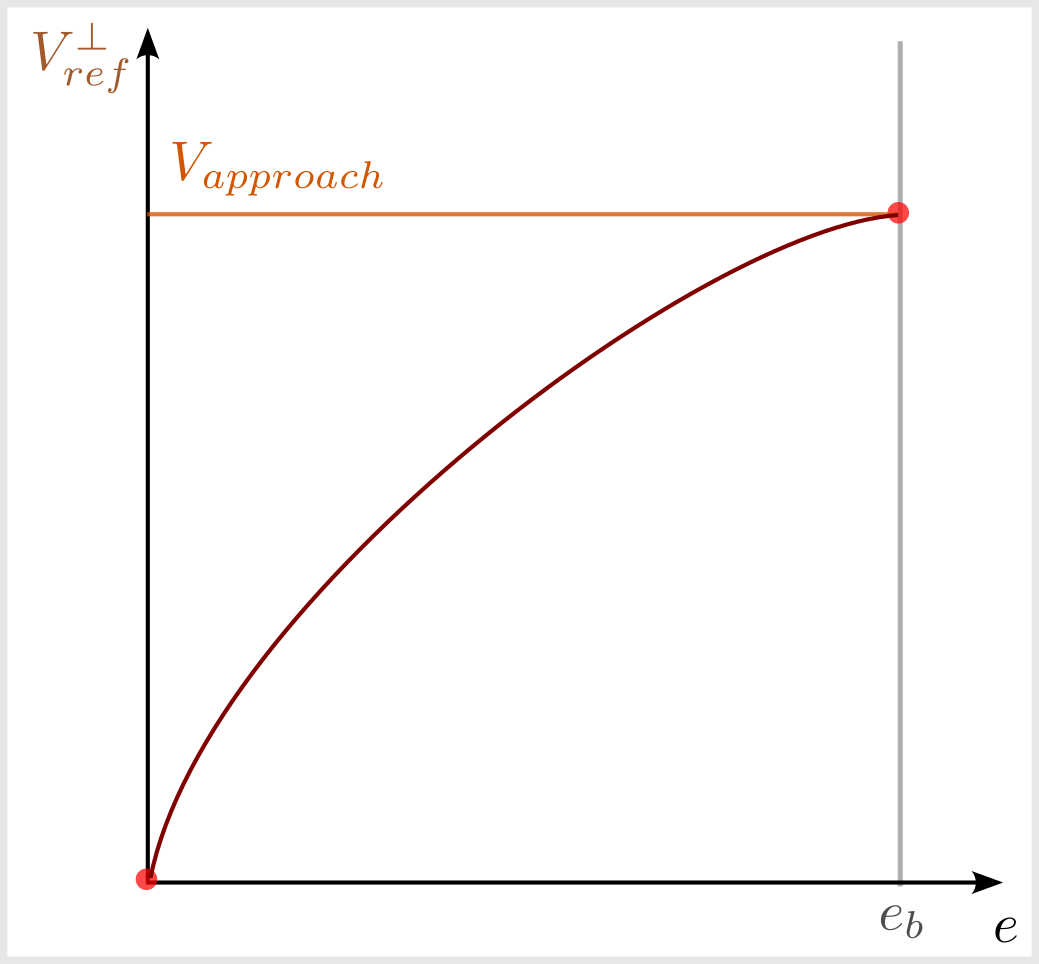
\includegraphics[width=0.5\textwidth]{V_orth_curve_v3.png}
\caption{\label{fig:v_orth_curve}Orthogonal Velocity Curve}
\end{figure}

Here, we define $V_{ref}^{\perp}(e)$, which represents the relationship between orthogonal velocity and cross-track error, as shown in \autoref{fig:v_orth_curve}.

\subsection{Constraints of $V_{ref}^{\perp}$}
To satisfy the entry and on-path conditions, it is clear that the orthogonal velocity curve has a constraint of:

\begin{equation}
%\[
V_{ref}^{\perp}(e)=\begin{cases}
    V_{approach}& \text{if $e = e_b$}\\
    0& \text{if $e = 0$}
\end{cases}
\label{eq:v_orth_constraints}
%\]
\end{equation}

Meaning that at the track error boundary,  approaching velocity must be respected and on path orthogonal velocity must be 0 (to follow the path).\newline

%%%%%%%%%% ACCEL LIMIT
\subsection{Acceleration limited orthogonal velocity profile}

\subsubsection{Derivations of orthogonal velocity curve}
Here is a more in-depth constraint formulation using derivation:

\begin{equation}
    \begin{split}
    \frac{d}{dt}V_{ref}^{\perp}(e) = \frac{de}{dt}\frac{d}{de}V_{ref}^{\perp}(e)\\
    = -V_{ref}^{\perp}(e) * \frac{d}{de}V_{ref}^{\perp}(e)
    \end{split}
\end{equation}

\begin{equation}
\begin{split}
    \text{Therefore, if } &\frac{d}{dt}V_{ref}^{\perp}(e) \geq -a^{\perp}_{max}\\
    &\frac{d}{de}V_{ref}^{\perp}(e) \leq \frac{a^{\perp}_{max}}{V_{ref}^{\perp}}
    \label{eq:accel_limit_orth_vel_deriv}
\end{split}
\end{equation}

This places an upper limit to the derivative of the $V_{ref}^{\perp}(e)$ curve.

\subsubsection{Simple maximum acceleration orthogonal velocity curve}
Using the constraint \autoref{eq:v_orth_constraints}, the 'maximum' acceleration (deceleration) profile of approaching the path can be defined like following:

\begin{equation}
    \text{With orthogonal acceleration limit: } a^{\perp}_{max}
\end{equation}

\begin{equation}
    S^{\perp}_{max-acc} = \{V_{ref}^{\perp}(e) | \ddot{e} = -a^{\perp}_{max}\}
\end{equation}

Where the $S^{\perp}_{max-acc}$ defines the most aggressive curve that is feasible (with a hard deceleration of $-a^{\perp}_{max}$ once the track error enters the track error boundary.\newline

This curve is in fact easily deducible using a constant acceleration equation on a 1-dimensional axis:

\begin{align}
    \text{With } e_b = \frac{V_{approach}^{2}}{2a^{\perp}_{max}}\\
    S^{\perp}_{max-acc}(e)=\begin{cases}
        \sqrt{2a^{\perp}_{max}} * \sqrt{e}& \text{if $e < e_b$}\\
        V_{approach}& \text{if $e \geq e_b$}
    \end{cases}
    \label{eq:s_orth_max_acc}
\end{align}

Particularly, we define the $e_b$ in this case as $e^{min}_{approach}$, which defines the \textbf{minimum required track error to bring $V_{approach}$ to 0 using maximum orthogonal acceleration}.

\begin{equation}
    e^{min}_{approach} = \frac{V_{approach}^{2}}{2a^{\perp}_{max}}
\end{equation}

\begin{figure}[h]
\centering
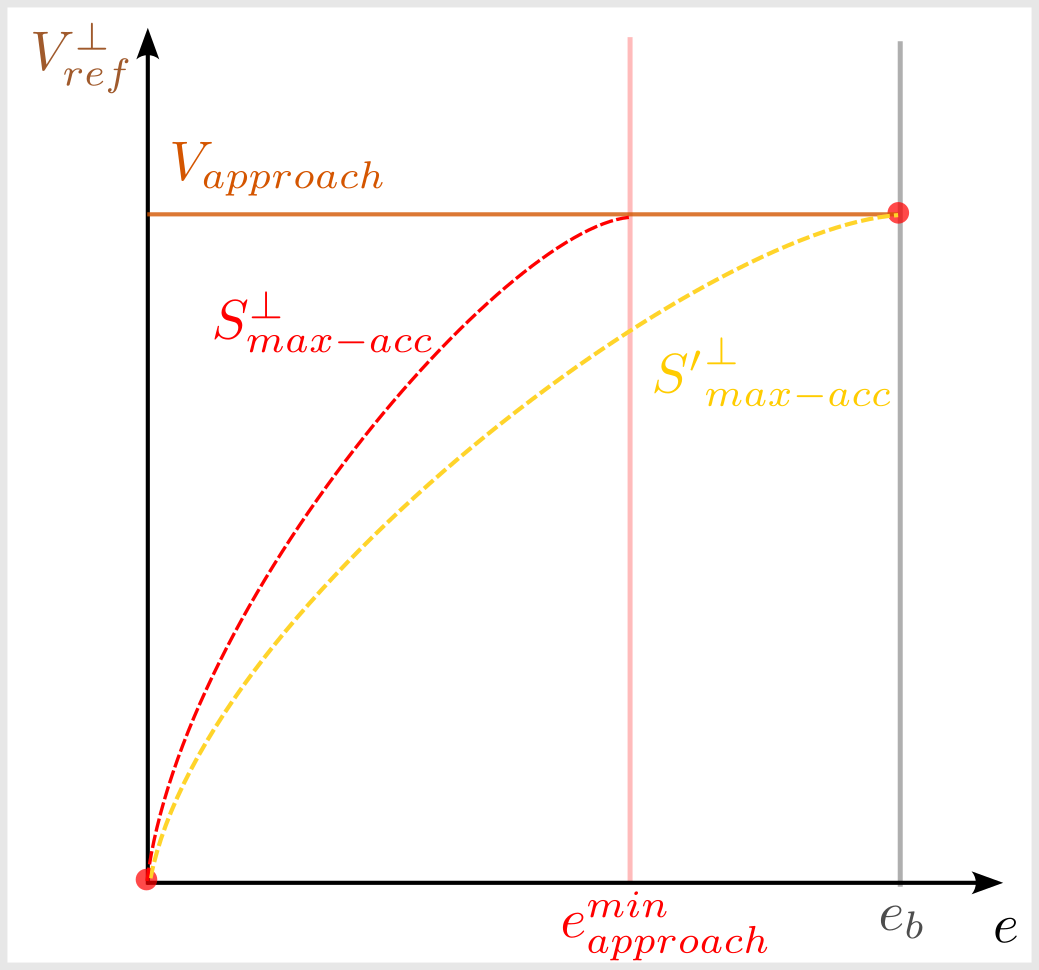
\includegraphics[width=0.5\textwidth]{S_orth_max_acc_v2.png}
\caption{\label{fig:s_orth_max_acc}Maximum orthogonal acceleration curve}
\end{figure}

Note here that $e^{min}_{approach}$ varies by acceleration limit and approach speed. And if we have a constant $e_b$ that we must satisfy (as drawn in \autoref{fig:s_orth_max_acc}), it is simply physically impossible to brake in time without overshooting the path if $e_b$ is smaller than $e^{min}_{approach}$. Therefore, another constraint applies:

\begin{equation}
    e_b \geq e^{min}_{approach}
    \label{eq:e_min_approach_e_b_constraint}
\end{equation}

And as long as the \autoref{eq:e_min_approach_e_b_constraint} and \autoref{eq:accel_limit_orth_vel_deriv} satisfies, \textit{any} curve can be a feasible curve that doesn't exceed maximum orthogonal acceleration limit.

%%%%%%%%%%%% RELAXED MAX ACCEL ORTH VEL
\subsubsection{Relaxed maximum acceleration orthogonal velocity curve}
As noted in the previous section, as long as the \autoref{eq:e_min_approach_e_b_constraint} satisfies, the velocity curve can be drawn. However, how do we actually accommodate the specified $e_b$ into the velocity curve?\newline

To provide a simple solution, a 'relaxed' orthogonal velocity curve  ${S'}^{\perp}_{max-acc}$ can be formulated like the following:

\begin{equation}
\begin{split}
    {S'}^{\perp}_{max-acc}(e) &= {S}^{\perp}_{max-acc}(\frac{e^{min}_{approach}}{e_b} * e)\\
    &=\begin{cases}
        \sqrt{\frac{2a^{\perp}_{max}e^{min}_{approach}}{e_b}} * \sqrt{e}& \text{if $e < e_b$}\\
        V_{approach}& \text{if $e \geq e_b$}
    \end{cases}\\
    &=\begin{cases}
        V_{approach} * \sqrt{\frac{e}{e_b}}& \text{if $e < e_b$}\\
        V_{approach}& \text{if $e \geq e_b$}
    \end{cases}
    \label{eq:relaxed_max_acc_orth_vel_curve}
\end{split}
\end{equation}

Which is basically a \textit{stretched} form of ${S}^{\perp}_{max-acc}$ to match $e^{min}_{approach}$ to specified $e_b$. This satisfies the acceleration derivative constraint (\autoref{eq:accel_limit_orth_vel_deriv}), because the derivative will always be below the upper limit when stretched across the track error axis. This is also illustrated in \autoref{fig:s_orth_max_acc}.\newline

Note that not \textit{every} curve between ${S}^{\perp}_{max-acc}$ and ${S'}^{\perp}_{max-acc}$ is a feasible curve. Because the derivative can go over the upper limit in local sections. Introducing the relaxed maximum acceleration orthogonal velocity curve was in fact motivated by the fact that there are infinite solutions, to provide a simple feasible solution.

%%%%%%%%%%%%%%%%%%%%%%%%%%%%%
% PARALLEL VEL
\section{Parallel Velocity Curve}
Now that we have a theoretical maximum acceleration constrained $V_{ref}^{\perp}(e)$ curve, the parallel Velocity curve can be defined.

% Need to be 400+ dpi to be smooth!
\begin{figure}[h]
\centering
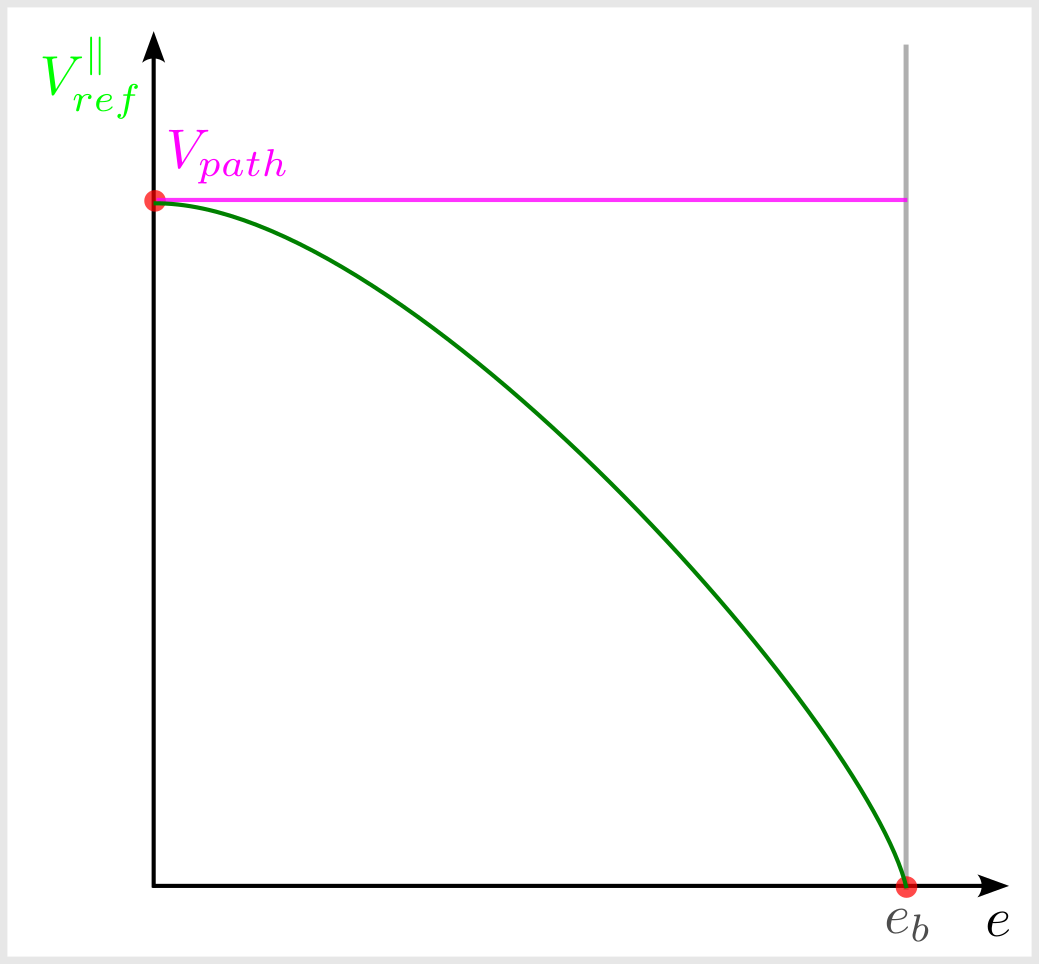
\includegraphics[width=0.5\textwidth]{V_parallel_curve_v3.png}
\caption{\label{fig:v_parallel_curve}Parallel Velocity Curve}
\end{figure}

\subsection{Constraints of $V_{ref}^{\parallel}(e)$}
To respect the boundary/on-path conditions, it is clear that the parallel velocity curve has a constraint of:

\begin{equation}
V_{ref}^{\parallel}(e)=\begin{cases}
    0& \text{if $e = e_b$}\\
    V_{path}& \text{if $e = 0$}
\end{cases}
\label{eq:v_parallel_constraints}
\end{equation}

\subsection{Acceleration limited parallel velocity profile}
First constraint that applies to $V_{ref}^{\parallel}(e)$ is it's acceleration along the direction parallel to the path. This can be derived easily, but with a dependency to orthogonal velocity curve.

\begin{equation}
    \text{With parallel acceleration limit: } a^{\parallel}_{max}
\end{equation}

\begin{equation}
    S^{\parallel}_{max-acc} = \{V_{ref}^{\parallel}(e) | \ddot{V}_{ref}^{\parallel}(e) = a^{\parallel}_{max}\}
\end{equation}

If we apply the derivation:

\begin{equation}
    \begin{split}
    \frac{d}{dt}V_{ref}^{\parallel}(e) = \frac{de}{dt}\frac{d}{de}V_{ref}^{\parallel}(e)\\
    = -V_{ref}^{\perp}(e) * \frac{d}{de}V_{ref}^{\parallel}(e)
    \end{split}
\end{equation}

% https://tex.stackexchange.com/questions/384299/splitting-lines-for-long-equations
\begin{equation}
\begin{split}
    \text{Therefore, if } &\frac{d}{dt}V_{ref}^{\parallel}(e) \leq a^{\parallel}_{max},\\
    &\frac{d}{de}V_{ref}^{\parallel}(e) \geq -\frac{a^{\parallel}_{max}}{V_{ref}^{\perp}(e)}
\end{split}
\end{equation}

This puts a lower bound on the derivative of $V_{ref}^{\parallel}(e)$, defining how aggressively the parallel velocity can decrease along cross-track error ($e$).\newline

%%%%%%%%%% Paralle velocity constraint with relaxed orth vel curve
\subsubsection{Maximum acceleration parallel velocity with relaxed max orthogonal velocity curve}
It should be noted that by substituting the relaxed maximum acceleration orthogonal velocity curve (\autoref{eq:relaxed_max_acc_orth_vel_curve}) to $V^{\perp}_{ref}(e)$, the constraint becomes:

\begin{equation}
\begin{split}
    \frac{d}{de}V_{ref}^{\parallel}(e) &\geq -\frac{a^{\parallel}_{max}}{{S'}^{\perp}_{max-acc}(e)}\\
    &=\begin{cases}
        -\frac{a^{\parallel}_{max}}{V_{approach}} * \sqrt{\frac{e_b}{e}}& \text{if $e < e_b$}\\
        -\frac{a^{\parallel}_{max}}{V_{approach}}& \text{if $e \geq e_b$}
    \end{cases}
\end{split}
\end{equation}

Also, considering boundary constraints in \autoref{eq:v_parallel_constraints}, it should be noted that another constraint must be satisfied between $V_{path}$ and $e_b$, since if the $V_{path}$ is too large, it would be impossible to reach the desired speed on path with a given $e_b$ distance to track. Therefore, we must compute the 'maximum' $V_{path}$ achievable with a given constraints:

\begin{equation}
    \begin{split}
        V_{path}^{max} |_{S'^{\perp}_{max-acc}} &= S^{\parallel}_{max-acc}(e=0)\\
        &= \int^{0}_{e_b}{-\frac{a^{\parallel}_{max}}{V_{approach}}\sqrt{\frac{e_b}{e}}} de\\
        &= -\frac{a^{\parallel}_{max}\sqrt{e_b}}{V_{approach}} * [2\sqrt{e}]^{0}_{e_b}\\
        &= \frac{2a^{\parallel}_{max}e_b}{V_{approach}}
    \end{split}
    \label{eq:max_path_speed_with_relaxed_orthog_speed_max_acc}
\end{equation}

Therefore, if $V_{path}$ is greater than the calculated $V_{path}^{max} |_{S'^{\perp}_{max-acc}}$, the parallel velocity curve is simply infeasible with the parallel acceleration constraints. And it is in fact possible to calculate the minimum track error boundary required to achieve the speed on path.

\begin{equation}
\begin{split}
    \text{Since } V_{path} &= \int_{e^{min}_{path}}^{0}-\frac{a^{\parallel}_{max}}{V_{approach}}\sqrt{\frac{e_b}{e}}de,\\
    &= -\frac{a^{\parallel}_{max}\sqrt{e_b}}{V_{approach}} * [2\sqrt{e}]^{0}_{e^{min}_{path}},\\
    \text{Therefore, } e^{min}_{path}|_{S'^{\perp}_{max-acc}} &= [\frac{V_{path}V_{approach}}{2a^{\parallel}_{max}}]^2*\frac{1}{e_b}
\end{split}
\end{equation}

Which defines the minimum track error point where acceleration in parallel velocity should be applied, with the given relaxed maximum acceleration orthogonal velocity curve $S'^{\perp}_{max-acc}$.\newline

Using this, we can formulate the maximum acceleration parallel velocity curve dependent on relaxed orthogonal velocity:

\begin{align}
    S^{\parallel}_{max-acc}(e)=\begin{cases}
        V_{path} - \frac{2a^{\parallel}_{max}\sqrt{e_b}}{V_{approach}} * \sqrt{e}& \text{if $e < e^{min}_{path}|_{S'^{\perp}_{max-acc}}$}\\
        0& \text{if $e \geq e^{min}_{path}|_{S'^{\perp}_{max-acc}}$}
    \end{cases}
    \label{eq:s_orth_max_acc}
\end{align}

\begin{figure}[h]
\centering
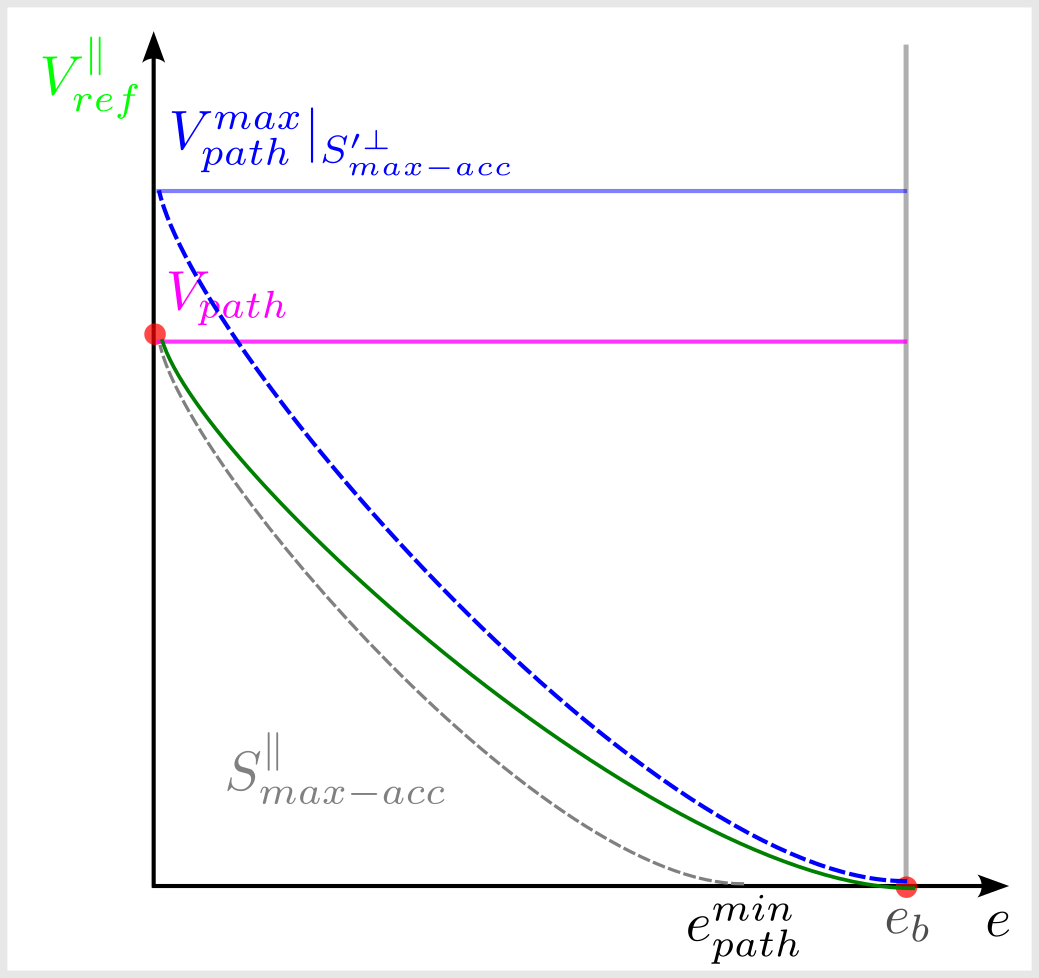
\includegraphics[width=0.5\textwidth]{S_parallel_max_acc_v2.png}
\caption{\label{fig:acc_limited_parallel_vel}Acceleration limited parallel velocity curve}
\end{figure}

\subsubsection{Relaxed parallel velocity curve with relaxed orthogonal velocity curve}
Similarly to orthogonal velocity curve's case, the $e^{min}_{path}|_{S'^{\perp}_{max-acc}}$ doesn't equal to $e_b$ all the time. Therefore, we introduce another relaxed parallel velocity curve that satisfies the acceleration limits:

\begin{equation}
\begin{split}
    {S'}^{\parallel}_{max-acc}(e) &= {S}^{\parallel}_{max-acc}(\frac{e^{min}_{path}|_{S'^{\perp}_{max-acc}}}{e_b} * e)\\
    &=\begin{cases}
        V_{path} - \frac{2a^{\parallel}_{max}\sqrt{e_b}}{V_{approach}} * \sqrt{\frac{e^{min}_{path}|_{S'^{\perp}_{max-acc}}}{e_b} * e}& \text{if $e < e_b$}\\
        0& \text{if $e \geq e_b$}
    \end{cases}\\
    &=\begin{cases}
        V_{path} * (1 - \sqrt{\frac{e}{e_b}})& \text{if $e < e_b$}\\
        0& \text{if $e \geq e_b$}
    \end{cases}
    \label{eq:relaxed_max_acc_parallel_vel_curve}
\end{split}
\end{equation}

This is a very similar form to \autoref{eq:relaxed_max_acc_orth_vel_curve}, as the velocities get ramped in/out proportional to $\sqrt{\frac{e}{e_b}}$.

\subsection{Velocity norm Monotonicity}
Another constraint is to make sure vehicle doesn't brake and accelerate, but rather have a constantly decreasing velocity norm profile when approaching path. This is desired since it gives a smooth speed curve, which can have higher efficiency (to be clarified), and more intuitive path following behavior.

\begin{equation}
    \dot{|V_{ref}|} \leq 0
\end{equation}

Since derivative of the velocity curves against track error ($e$), when multiplied by $-V^{\perp}_{ref}$ gives the derivative against time, this can be formulated as:

\begin{equation}
    \begin{split}
        \dot{|V_{ref}|} &= \dot{\sqrt{{V_{ref}^{\parallel}}^2 + {V_{ref}^{\perp}}^2}}\\
        &= \frac{1}{|V_{ref}|} * (\dot{V}_{ref}^{\parallel} + \dot{V}_{ref}^{\perp})\\
        &= \frac{-V^{\perp}_{ref}}{|V_{ref}|} * (\frac{{dV}_{ref}^{\parallel}}{de} + \frac{{dV}_{ref}^{\perp}}{de})\\
        \text{Therefore, } &\frac{{dV}_{ref}^{\parallel}}{de} + \frac{{dV}_{ref}^{\perp}}{de} \geq 0
    \end{split}
\end{equation}

\subsubsection{Monotonicity constraint on relaxed curves}
Using \autoref{eq:relaxed_max_acc_orth_vel_curve} and \autoref{eq:relaxed_max_acc_parallel_vel_curve}:

\begin{equation}
\begin{split}
    \frac{{dV}_{ref}^{\parallel}}{de} + \frac{{dV}_{ref}^{\perp}}{de} = \frac{V_{approach}-V_{path}}{\sqrt{e_b}} * \frac{1}{2\sqrt{e}} \geq 0
\end{split}
\end{equation}

This indicates that for our relaxed curves to satisfy monotonically reducing velocity form as it approaches the path, the approach velocity must be bigger than velocity on path.